
\documentclass[dvisvgm]{standalone}
\usepackage{tikz}

\usetikzlibrary {arrows.meta,automata,positioning,shapes.geometric}
        

\begin{document}

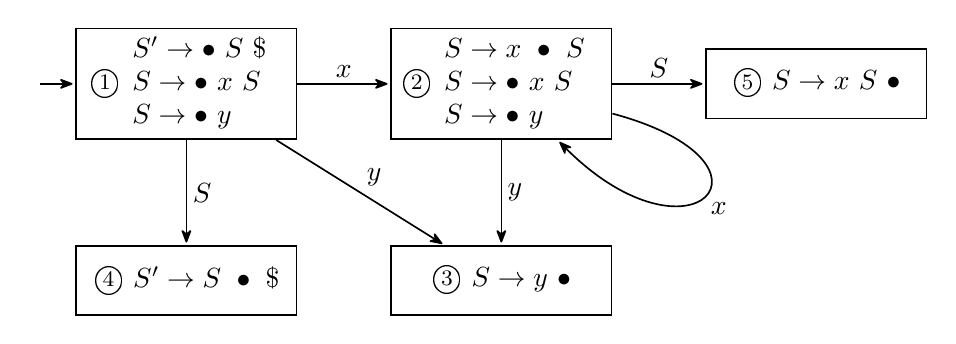
\begin{tikzpicture}[->,>={Stealth[round]},shorten >=1pt,auto,node distance=4cm,on grid,semithick,inner sep=2pt,bend angle=50,initial text=,every state/.style={draw,rectangle,minimum width=2.8cm}]
\node[initial,state] (q_1) {\textcircled{\footnotesize 1}\!\begin{tabular}{l} $S'\to\bullet\ S\ \$$ \\ $S\to\bullet\ x\ S$ \\ $S\to\bullet\ y$ \end{tabular}};
        \node[state] at (4, 0) (q_2) {\textcircled{\footnotesize 2}\!\begin{tabular}{l} $S\to x\ \bullet\ S$ \\ $S\to\bullet\ x\ S$ \\ $S\to\bullet\ y$ \end{tabular}};
        \node[state] at (4, -2.5) (q_3) {\textcircled{\footnotesize 3}\ $S\to y\ \bullet$};
        \node[state] at (0, -2.5) (q_4) {\textcircled{\footnotesize 4}\ $S'\to S\ \bullet\ \$$};
        \node[state] at (8, 0) (q_5) {\textcircled{\footnotesize 5}\ $S\to x\ S\ \bullet$};
        \path
            (q_1) edge node {$x$} (q_2)
                  edge node {$y$} (q_3)
                  edge node {$S$} (q_4)
            (q_2) edge node {$S$} (q_5)
                  edge node {$y$} (q_3)
                  edge [in=-45,out=-15,loop] node {$x$} (q_2);
\end{tikzpicture} 


\end{document}
